Meshes are fundamental tools in Finite Element algorithms. This particular algorithm utilizes polygonal meshes over a polygonal domain.

\begin{figure}[!ht]
	\centering
	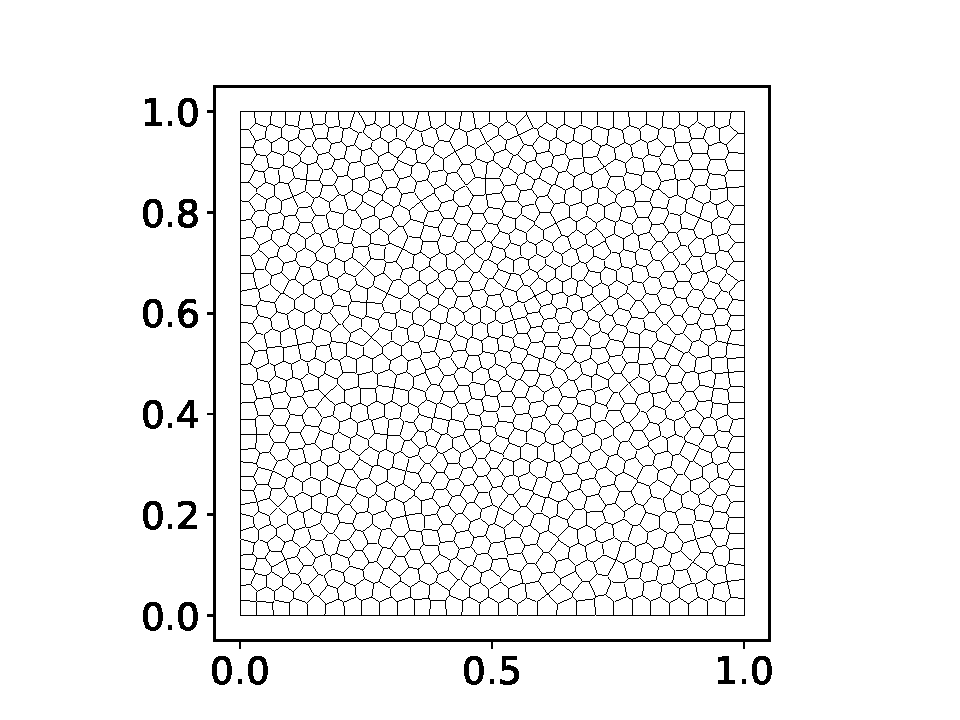
\includegraphics[trim=0cm 0.5cm 0cm 0.5cm, clip, width=7.5cm]{meshes/uniform/square_1000.pdf}
    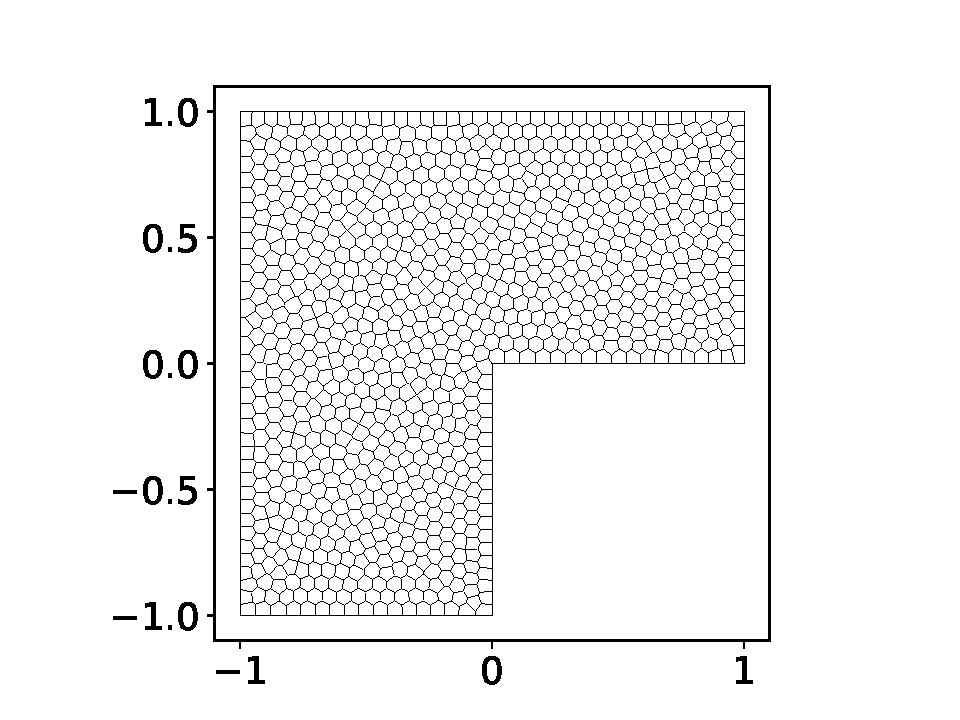
\includegraphics[trim=0cm 0.5cm 0cm 0.5cm, clip, width=7.5cm]{meshes/uniform/lshape_1000.pdf}
	\caption{Square and L-shaped meshes over polygonal domains, $N = 1000$.}
\end{figure}

\cite{Talischi2012} The mesh-building strategy follows these steps:

\begin{enumerate}
	\item Evaluate the Voronoi diagram.
	\item Perform relaxation using the Lloyd algorithm.
	\item Collapse excessively small edges.
	\item Assess the neighboring structure.
	\item Compute mesh properties, including element areas and largest simplices.
\end{enumerate}

The \lstinline{mesh_diagram} function requires a polygon (serving as the mesh's domain), a number of points (determining how many points are generated inside the polygon), and a reflection flag (which instructs the \lstinline{voronoi} function to reflect each point relative to the polygon's boundary and vertices to accommodate non-convex polygons). The function evaluates each cell by starting with the polygon\footnote{For non-convex domains, the initial cell is the bounding box.} as the initial cell for a point, then reduces it with respect to every other point using their respective bisectors. This process continues using Lloyd's algorithm.

Diagrams are then post-processed to collapse excessively small edges while preserving their overall shape and properties, and to correct any errors caused by reflection.

After post-processing, the mesh is prepared by evaluating each element within the diagram, assessing the neighboring structure, and computing various properties of the mesh, such as the areas of the elements and the largest simplices.

\newpage
\subsection{A code snippet}

Here's a snippet to illustrate the mesh building process from the user's perspective:

\lstinputlisting[style=cpp, firstline=11]{../snippets/square_mesh.cpp}